\chapter{Antecedentes}
\label{chap:antecedentes}


%%%%%%%%%%%%%%%%%%%%%%%%%%%%%%%%%%%%%%%%%%%%%%%%%%%%%%%%%%%%%%%%%%%%%%%%%%%%%%%%
% Objetivo: Contar cómo estaba la situación antes de empezar,                  %
%           t0do lo que se hizo para familiarizarse con las tecnologías,       %
%           casarlas, etc.                                                     %
%%%%%%%%%%%%%%%%%%%%%%%%%%%%%%%%%%%%%%%%%%%%%%%%%%%%%%%%%%%%%%%%%%%%%%%%%%%%%%%%
%todo http://humanrobotinteraction.org/human-robot-interaction-a-historical-perspective-and-current-research-trends/


%Objetivos de interacción del proyecto, modelo conceptual del mismo.

\lettrine{E}{n} este capítulo se introduce el tema de la Interacción humano robot, 	y el diseño conceptual del sistema de interacción desarrollado para la plataforma ROBOBO.

\section{Interacción humano robot}
 \label{sec:hri-intro}
 
 %todo meter lo de las conferencias
 Desde finales de la década de los 90, la interacción entre humanos y robots ha cobrado importancia, creando un nuevo campo de investigación en la ciencia\cite{goodrich2007human}, la interacción humano-robot (HRI por sus siglas en inglés). El campo de la HRI busca entender, modelar y evaluar las diferentes modalidades de interacción entre las personas y los robots. La comunicación entre humanos y robots puede dividirse  en dos categorías generales:
 \begin{itemize}
 	\item Interacción remota
 	\item Interacción próxima
 \end{itemize}
 
 La interacción remota suele ser referida como control supervisado o teleoperación, dependiendo de si el robot es autónomo con supervisión de un humano, que interviene en caso de necesidad, o si el robot es controlado por el humano directamente. Este tipo de interacción puede verse en robots de tipo industrial o en vehículos autónomos, cómo los llamados Drones del ejército.
 
 La interacción próxima es aquella en la que el robot interactúa directamente con el humano, llegando incluso a haber interacción física. Este tipo de interacción incluye elementos emotivos y sociales, y se puede encontrar en, por ejemplo, los robots asistenciales o educativos. Este tipo de interacción es la que se tratará en este trabajo, en el cual se diseñarán diferentes sistemas de interacción para la plataforma ROBOBO.
 
 \subsection{HRI en la industria}
 
 Generalmente, en los procesos industriales, la interacción entre los robots y los operadores suele ser remota, los sistemas se programan para realizar una tarea y el humano solamente interviene en caso de necesidad, sin embargo pueden darse casos de interacción próxima con los robots. Uno de estos casos podría ser el aprendizaje de tareas mediante demostración, proceso mediante el cual, un operador humano realiza una tarea, por ejemplo moviendo manualmente el brazo de un robot, para que el controlador aprenda a realizar esa tarea. Este tipo de interacción permite que los robots aprendan comportamientos de alto nivel difícilmente programables.
 
 Sin embargo a la hora de realizar tareas de forma cooperativa entre robots y humanos, la interacción cercana con robots industriales conlleva riesgos importantes, como pudo verse en el accidente del 2015\cite{vwaccident2015} en la planta de Volkswagen cerca de Kassel, Alemania, en el que un operario fue golpeado por un brazo industrial  durante su instalación, resultando en la muerte del técnico.
  \begin{figure}
	\centering
	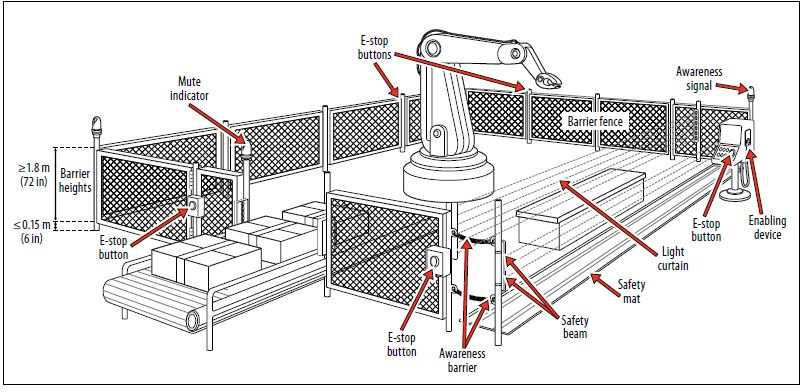
\includegraphics[width=1\linewidth]{imagenes/robotcell.jpeg}
	\caption{Esquema de una jaula de seguridad para un robot industrial}
	\label{fig:robot-cell}
\end{figure} 
 Para evitar esta clase de accidentes, se está buscando la consciencia del entorno en los manipuladores robóticos, para poder adaptar sus reacciones al contexto actual. Este tipo de consciencia no solo disminuye los riesgos de operación, sino que también disminuye los costes espaciales, ya que los robots no requerirían de jaulas de seguridad (figura \ref{fig:robot-cell}), también la productividad se vería afectada positivamente, ya que tareas imposibles de realizar para un robot y para un humano individualmente, pueden llevarse a cabo mediante la llamada robótica cooperativa.
 En \textit{Cooperative Tasks between Humans and Robots in Industrial Environments}\cite{corrales2012cooperative} presentan un sistema de robótica cooperativa en el que un operador y un robot colaboran de manera cercana para llevar a cabo diferentes tareas, de manera que el robot realiza las tareas repetitivas y peligrosas, mientras que el humano lleva a cabo las tareas que requieren de cierta precisión o inteligencia con la que no cuenta el robot. En este sistema el operador lleva un traje de posicionamiento, que permite al robot conocer su posición, pudiendo así adaptar sus movimientos de manera que el humano no corra riesgos.
 
 
 
 \subsection{HRI en robots asistenciales}
 Uno de los campos en los que la interacción entre humanos y robots cobra mucha importancia es en el nicho de los robots asistenciales. Los robots asistenciales, también llamados de servicio, son definidos por la federación internacional de robótica cómo \textit{Robots que operan de forma total o semiautónoma para realizar servicios útiles para el bienestar de humanos y equipamiento, excluyendo las operaciones de manufactura}\cite{ifr-service-robots}. En esta definición se diferencia entre dos tipos de robots asistenciales:
 \begin{itemize}
 	\item Robots personales
 	\item Robots profesionales
 \end{itemize}
 
 Los robots personales son aquellos que se utilizan para labores no comerciales, generalmente por personas sin perfil técnico. Por ejemplo, sillas de ruedas eléctricas, robots de asistencia de movilidad, o aspiradoras automáticas.
 
 Los robots profesionales son aquellos utilizados para realizar tareas de asistencia en un entorno comercial, generalmente manejados y supervisados por un personal especializado. Por ejemplo robots de limpieza automatizados para zonas públicas, robots de mensajería en oficinas u hospitales, robots anti-incendios,robots quirúrgicos y de rehabilitación en hospitales o los robots terapéuticos.
 \begin{figure}
	\centering
	
\includegraphics[width=0.8\linewidth]{imagenes/parorobot.JPG}
	\caption{Robot terapeutico Paro}
	\label{fig:parorobot}
\end{figure} 

 En los robots terapéuticos se pueden encontrar múltiples formas de interacción, por ejemplo, el robot Paro\cite{parorobots} (figura \ref{fig:parorobot}) es un robot terapéutico con forma de bebé foca, utilizado con éxito en terapias contra la Demencia, que busca una interacción emocional con el paciente, para ello cuenta con cinco tipos de sensores diferentes, táctiles, auditivos, de temperatura, de luz y posturales. Los pacientes realizan una interacción con el robot cómo la que tendrían con un animal, y el robot responde acorde a los estímulos que recibe. Esto, en conjunto con la forma física del robot, más semejante a un animal de peluche que a una máquina, permite al paciente desarrollar emociones.
   \begin{figure}
	\centering
	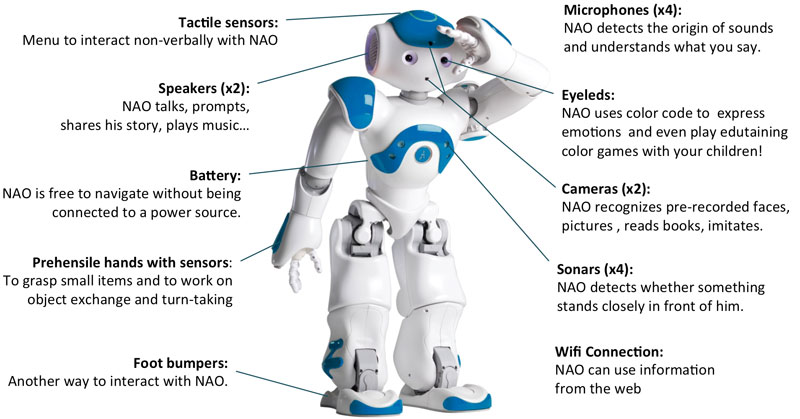
\includegraphics[width=1\linewidth]{imagenes/naorobot.jpg}
	\caption{Esquema de características del robot NAO}
	\label{fig:naorobot}
\end{figure} 
 El robot NAO\cite{naorobots}(figura \ref{fig:naorobot}) es otro de los robots que se están empleando con éxito en tareas asistenciales, tanto de manera terapéutica, como robot de relaciones publicas o para tareas de educación. El robot cuenta con una amplia variedad de sensores y actuadores que le permiten interactuar de diversas formas con el usuario:
 \begin{itemize}
 	\item Cámaras: Permiten reconocimiento de caras y procesado de imagen.
 	\item Sensores táctiles y de presión: Permiten una interacción física con el robot.
 	\item Altavoces: Permiten al robot producir diversos sonidos y hablar.
 	\item Micrófonos: Permiten reconocer habla y ubicar el origen de los sonidos espacialmente.
 	\item Sensores de distancia: Permiten detectar la distancia a los objetos.
 	\item 25 Grados de libertad: Permiten al robot interactuar fisicamente con su entorno y realizar comunicación no verbal.
 	\item Unidad de medición inercial: Permite detectar aceleraciones y giros.
 \end{itemize}
\begin{figure}
	\centering
	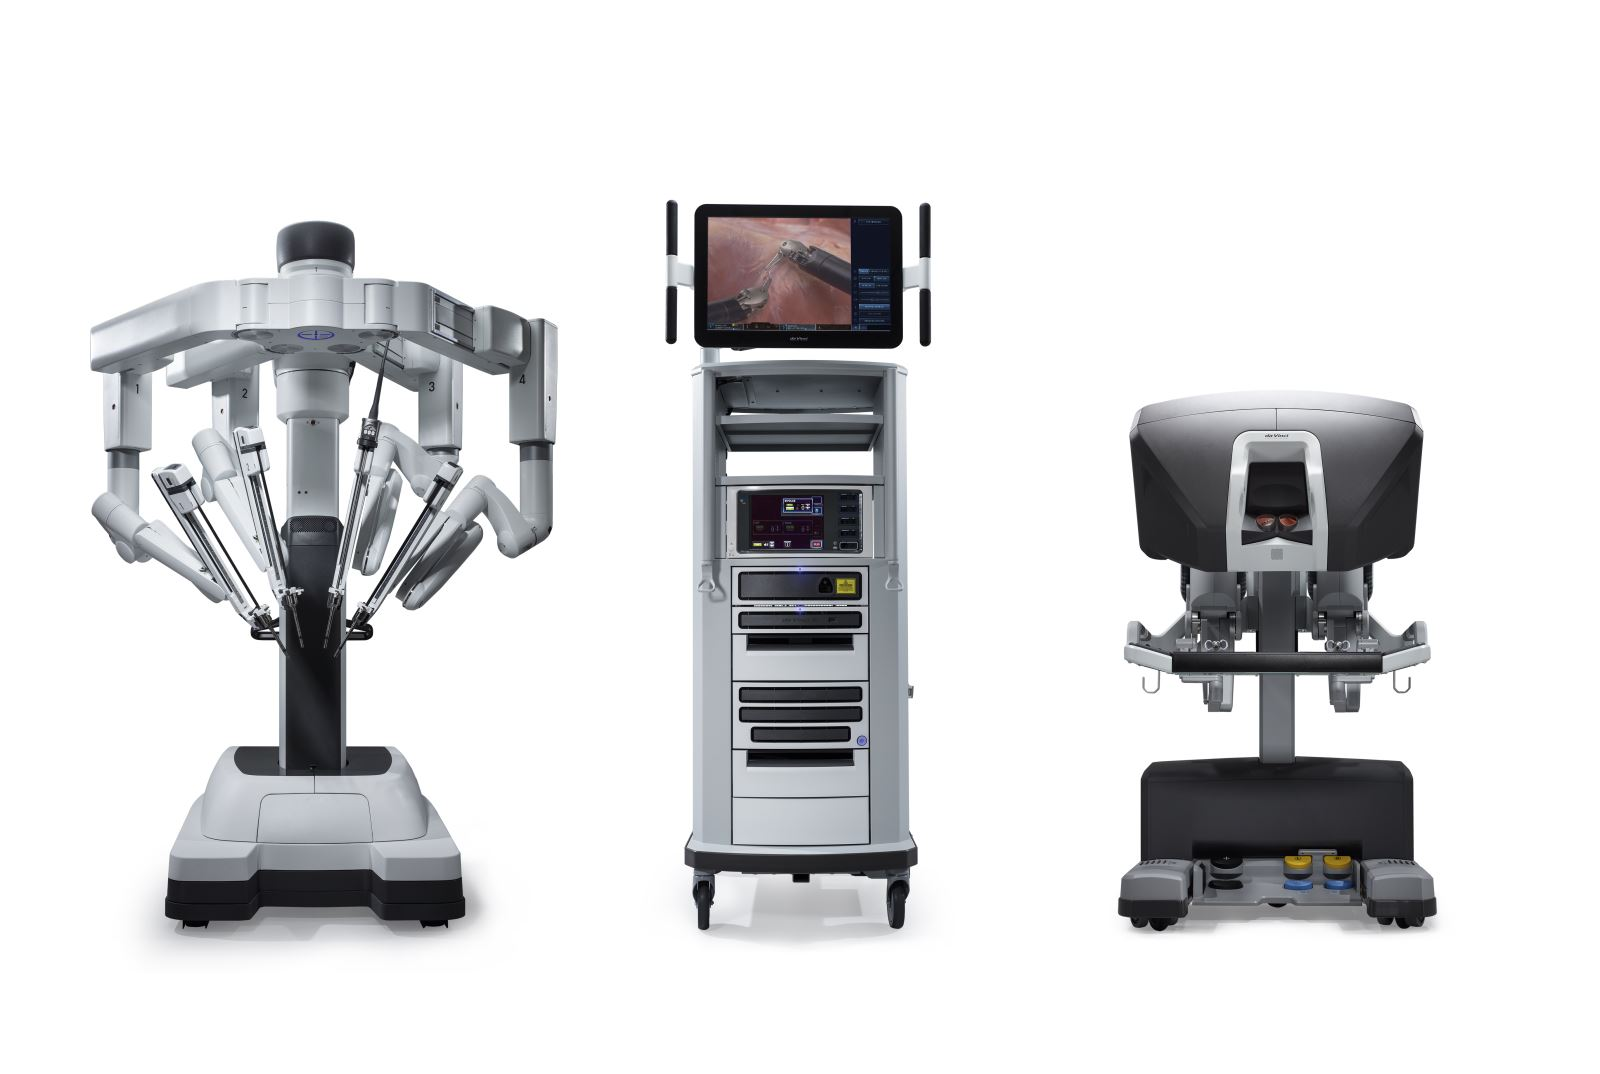
\includegraphics[width=1\linewidth]{imagenes/davincisystem.jpg}
	\caption{Sistema quirúrgico daVinci}
	\label{fig:davincisystem}
\end{figure} 
 
 En el caso de los robots médicos, los quirúrgicos especificamente, la interacción no suele pasar de la teleoperación del robot, es decir, el robot se controla como si fuera una extensión del cirujano. El robot más conocido en este campo es el sistema quirúrgico Da Vinci (figura \ref{fig:davincisystem}), utilizado en cirugía de precisión. En este robot el cirujano controla los diferentes brazos del aparato desde una consola que cuenta con controles con feedback háptico, es decir, el operador no solamente mueve el brazo, sino que siente lo que hay al final del mismo, la presión ejercida y la resistencia al movimiento, dando al cirujano el tacto necesario para realizar las diferentes tareas que se realizan en una operación, como coser o cortar, de forma natural y con un alto grado de precisión, ya que permite escalar los movimientos del cirujano.
 

 
 \subsection{HRI en robots de entretenimiento}
 Se entiende por robots de entretenimiento aquellos cuya finalidad no es más que divertir al usuario. Dentro de esta categoría podríamos incluir a los robots mascota, que generalmente realizan una interacción de alto nivel con el usuario.
 Por ejemplo, uno de los robots más relevantes en el ámbito de los robots mascota es el desarrollado por Sony, Aibo \cite{aibo} (figura \ref{fig:aiborobot}) , cuya finalidad era comportarse como un perro. En este robot podemos encontrar múltiples tipos de interacción, interacción física en forma de movimientos perrunos, reconocimiento facial a través de cámaras, a través de caricias utilizando los sensores táctiles, y en las últimas versiones del robot mediante una matriz de leds situada en la cara del aparato, que permite poner diferentes expresiones en función del "humor" del robot. Mediante todas estas capacidades motoras y sensoriales, se puede interactuar con una unidad Aibo de manera semejante a la que se tendría con un perro real.
 Otro ejemplo de mascota robótica es el Bandai SmartPet (figura \ref{fig:bandaismartpet}) , un robot pensado para utilizar junto un smartphone IPhone, que es colocado en la cabeza del robot y provee múltiples formas de interacción, reconocimiento de gestos mediante la cámara frontal, reconocimiento de sonido utilizando el micrófono y reconocimiento de gestos táctiles en la pantalla.
 
 \begin{figure}
	\centering
	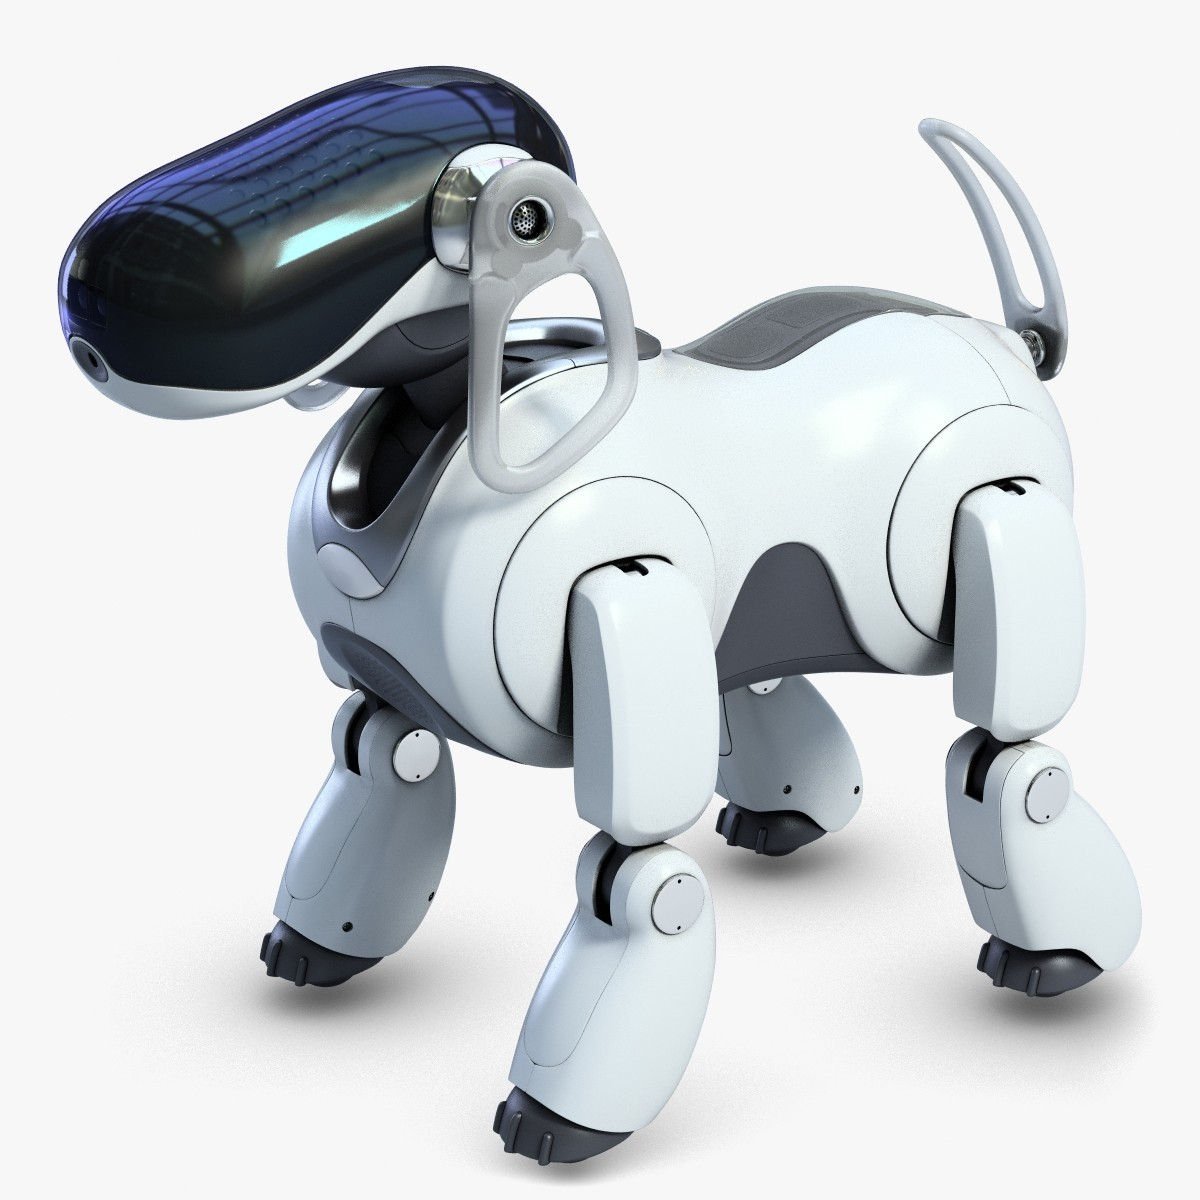
\includegraphics[width=0.5\linewidth]{imagenes/aiborobot.jpg}
	\caption{Robot mascota Aibo de Sony}
	\label{fig:aiborobot}
 \end{figure}
  \begin{figure}
	\centering
	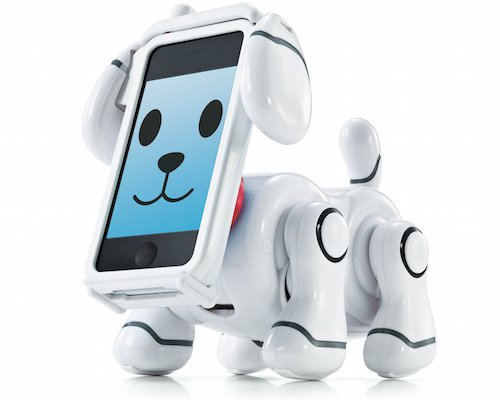
\includegraphics[width=0.5\linewidth]{imagenes/bandaismartpet.jpg}
	\caption{Robot mascota Smartpet de Bandai}
	\label{fig:bandaismartpet}
 \end{figure}

 \subsection{HRI en robots educativos}
 En  los últimos años el uso de robots con fines educativos, si bien ya eran usados de manera educativa en enseñanza superior, ha tomado impulso en la educación primaria y secundaria, apareciendo múltiples robots enfocados a este tipo de mercado. La interacción con esta clase de robots puede darse de diferentes formas según el público objetivo, dependiendo principalmente del rango de edades del mismo.

\begin{figure}
\centering
\begin{minipage}{0.45\textwidth}
\centering
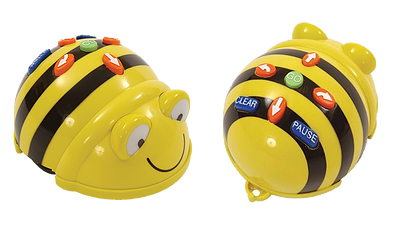
\includegraphics[width=1\linewidth]{imagenes/beebot.png}
\caption{Beebot}
\label{fig:beebot}

\end{minipage}\hfill
\begin{minipage}{0.45\textwidth}
\centering
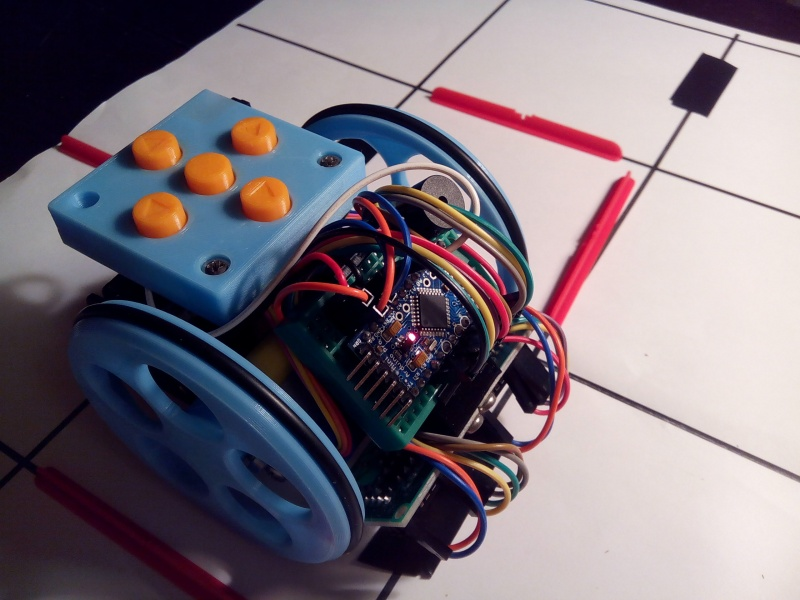
\includegraphics[width=1\linewidth]{imagenes/escornabot.jpg}

\caption{Escornabot}
\label{fig:escornabot}

\end{minipage}
\end{figure}

 Enfocados a la educación infantil nos podemos encontrar con robots cómo el BeeBot(figura \ref{fig:beebot}) o su alternativa libre, el Escornabot(figura \ref{fig:escornabot}), el cometido de estos robots es introducir los niños a la programación, en forma de pensamiento secuencial, y a la resolución de problemas. En esta clase de robots la interacción está limitada a la introducción de comandos en la botonera de la parte superior del robot, que serán traducidos a movimientos del robot posteriormente.  

 En la educación primaria y secundaria los robots utilizados ya adquieren una mayor complejidad y suelen emplearse para una introducción real a la programación, generalmente utilizando lenguajes gráficos de muy alto nivel como Scratch\cite{scratch}. Uno de los robots más relevantes en este ámbito es el kit Mindstorms de Lego (figura \ref{fig:legoev3}) , que no solo permite programar el robot, sino también construirlo. El Lego Mindstorms cuenta con diferentes sensores y actuadores que ofrecen diversas maneras de interacción con el robot:
 \begin{itemize}
 	\item Motores: Permiten el movimiento del robot de manera relativamente precisa
 	\item Sensores de distancia: Permiten medir distancias y actuar en consecuencia a los datos medidos
 	\item Sensores de luz ambiente: Miden la intensidad de la luz del entorno
 	\item Sensores de color: Permiten detectar los colores básicos
 	\item Unidad inercial: Permite medir giros en el plano horizontal
 \end{itemize}
 
   \begin{figure}
	\centering
	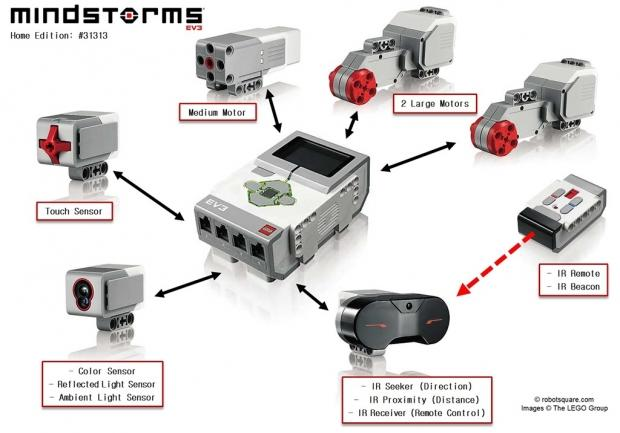
\includegraphics[width=0.8\linewidth]{imagenes/legoev3.jpg}
	\caption{Kit básico Lego Mindstorms EV3}
	\label{fig:legoev3}
\end{figure} 

En la llamada educación especial la robótica también está siendo empleada con éxito, por ejemplo el robot NAO (figura \ref{fig:naorobot}), del que se habló en la sección anterior, se utiliza para educar a niños con trastornos de espectro autista. El éxito de este tipo de educación viene dada debido a que la interacción con el robot, al ser programada, resulta predecible para el alumno, creando un entorno estable y pautado que resulta óptimo en este tipo de trastornos. La interacción en este caso se da en forma de movimientos preprogramados y mediante los leds de los ojos del robot, que cambian de color según las emociones que intenta expresar el robot, lo cual ayuda al alumno a ejercitar uno de las mayores dificultades dadas por el autismo, la dificultad de establecer relaciones empáticas.
 %todo continuar esto mirar mail de gervasio
 

 
   \begin{figure}
	\centering
	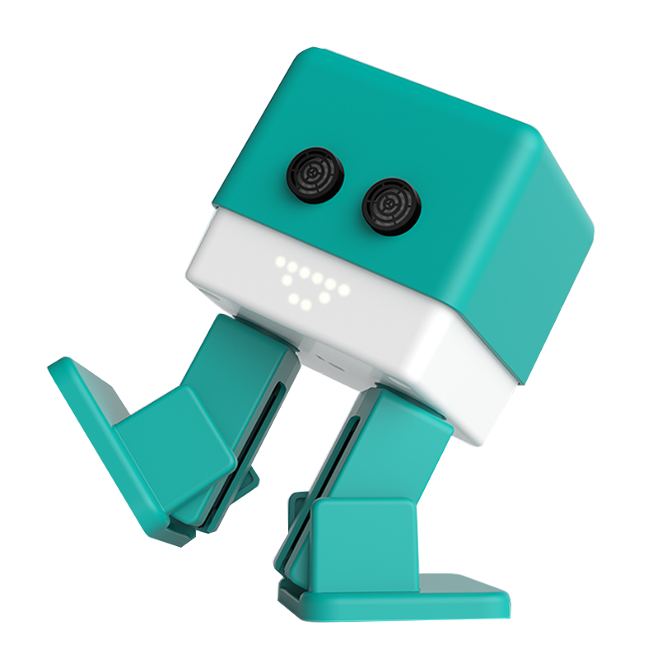
\includegraphics[width=0.6\linewidth]{imagenes/zowi.png}
	\caption{Robot Zowi de BQ}
	\label{fig:zowi}
\end{figure} 

 Entre otros ejemplos de robots educativos podemos encontrar el Zowi(figura \ref{fig:zowi}) de la empresa española BQ. Zowi es un robot educativo enfocado a niños, cuanta con un sensor de ultrasonidos para medir distancias, un micrófono que le permite detectar sonidos, una pequeña matriz de leds a modo de boca, que permite comunicarse mediante expresiones faciales, y con cuatro servos posicionados en forma de dos piernas que permiten moverse al robot.
 El robot viene con varios juegos para niños instalados de serie, y cuanta además con una aplicación de control para smartphones. Zowi puede ser empleado para enseñar programación a niños con un lenguaje gráfico similar a Scratch\cite{scratch}, Bitbloq\cite{bitbloq}.
 
  \begin{figure}
	\centering
	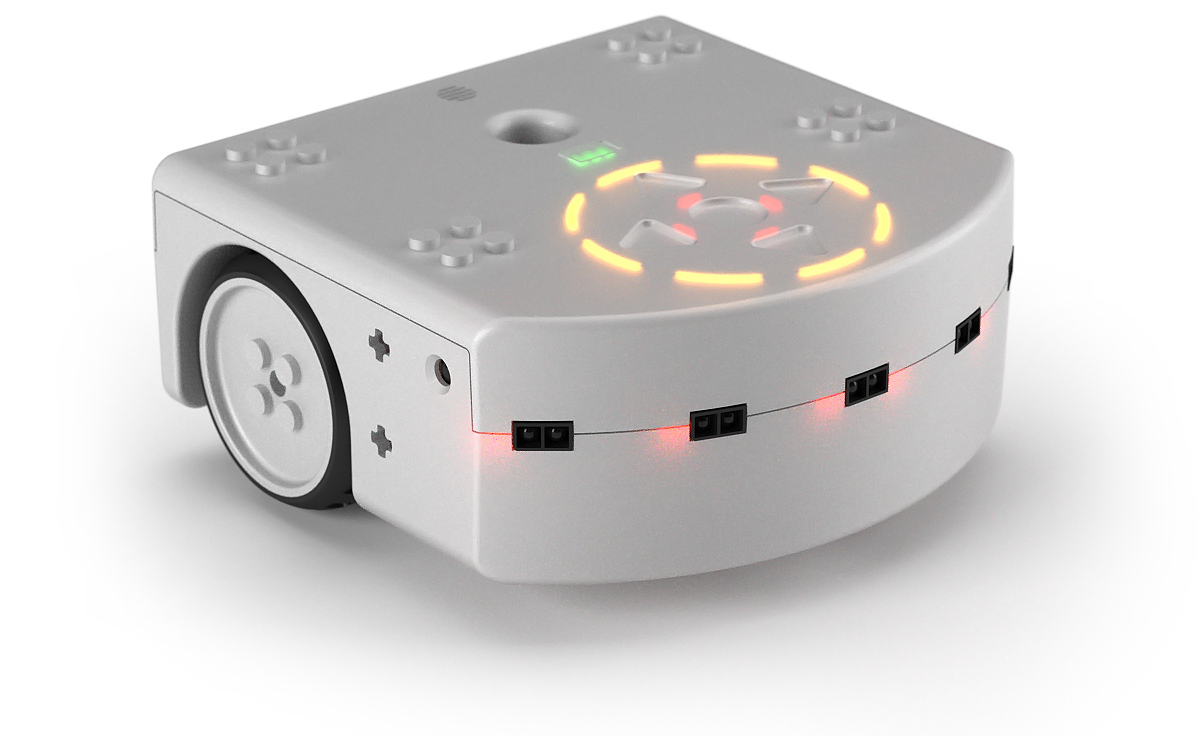
\includegraphics[width=0.6\linewidth]{imagenes/tymio.jpg}
	\caption{Robot Thymio}
	\label{fig:thymio}
\end{figure} 
 Otro robot educativo es el Thymio(figura \ref{fig:thymio}). Este robot cuenta con gran variedad de sensores, de distancia, acelerómetros, temperatura, control por infrarrojos, seguidores de lineas y micrófono, y con dos ruedas compatibles con las piezas de lego. La interacción con el usuario se realiza a través de los 39 leds RGB situados por todo el chasis, 5 teclas capacitivas que se encuentran en la parte superior del robot y los sensores citados anteriormente. El robot está pensado para enseñar programación a los niños de diferentes rangos de edad, para ello se pueden emplear 3 lenguajes diferentes de programación, Visual Programming Language (VPL) para los niños a partir de 6 años, Blockly, un lenguaje de programación gráfico semejante a Scratch desarrollado por Google, para niños a partir de 9 y programación textual mediante el software Aseba Studio para niños a partir de 12 años.
 
 Dash and Dot (figura \ref{fig:dashanddot}) son una pareja de robots educativos fabricados por Wonder Workshop enfocados a niños de poca edad. Dash cuenta con una plataforma motorizada equipada con sensores de distancia,\enquote{orejas} motorizadas, tres micrófonos, un altavoz, un \enquote{ojo circular} con 12 leds blancos, leds rgb en las \enquote{orejas} y \enquote{pecho}. Dot en cambio, es una alternativa más económica que solo incluye la \enquote{cabeza} de Dash. Gracias a la gran cantidad de actuadores, Dash, y en menor medida Dot, cuentan con diversas formas de interacción con los niños, desde el movimiento del robot, habla a través del altavoz,  gestos con los leds del ojo e incluso, mediante accesorios vendidos de forma separada, tocando un pequeño xilófono o lanzando pelotas con una pequeña catapulta, Dot además cuenta con un accesorio \enquote{orejas de conejo} que le permite suplir la falta de plataforma motorizada y moverse. Estos robots están pensados para enseñar programación a los niños, y cuentan con varias aplicaciones diseñadas para este cometido, \textit{Path}, que permite a los niños dibujar la ruta que desean que tome el robot, \textit{Wonder}, un lenguaje visual de programación y \textit{Blockly}, el lenguaje de programación por bloques desarrollado por Google.
 
   \begin{figure}
	\centering
	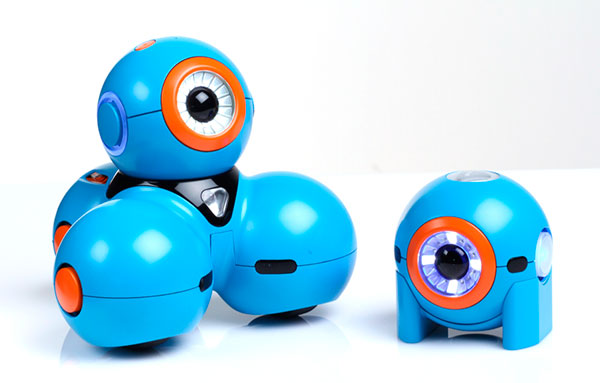
\includegraphics[width=0.6\linewidth]{imagenes/dashanddot.jpg}
	\caption{Robots Dash y Dot}
	\label{fig:dashanddot}
\end{figure} 
 
 
 \subsection{Conclusión}
   
Cómo se pudo apreciar en las secciones anteriores de este capítulo, el campo de la interacción humano robot es amplio y crucial en la evolución de la robótica por ello el desarrollo de nuevas formas de interacción permitirá el avance y la implantación de la misma en ámbitos generales de la sociedad, sin limitarse a nichos como puede ser la industria o la educación.
En el ROBOBO, se tomarán como ejemplos alguno de los robots comentados anteriormente para desarrollar un sistema de HRI completo y funcional que permita una interacción fluida con el robot.

 

   
